\chapter[System Description]{System Description}
\label{chap:descricaoproblema}


\section{Processo de Fazer Alguma Coisa}
\label{sec:hist}

Cada seção inicia pela descrição do seu conteúdo e pode terminar com um parágrafo de conexão com a seção seguinte. 

Antes de formular o problema, \textbf{não se esqueça de fazer todas as definições necessárias}. Também devem-se detalhar os aspectos complementares da abordagem: se estamos estudando um aspeto particular do problema, se a resposta encontrada é universal ou dependente de simplificações e hipóteses prévias.


\section{Instrumentação do Processo}
\label{sec:instrumentação}

Descreva a aparelhagem e o equipamento utilizados bem como a ligação entre os diversos componentes. Nesta seção e, ao longo de todo o texto, você deve dar detalhes suficientes para que qualquer pessoa consiga reproduzir seus experimentos.

Contudo, \textbf{não disperse o leitor com detalhes irrelevantes} ou aspectos
demasiado técnicos ou formais. Reserve tais detalhes para um
apêndice.

ilustramos o processo com a Figura \ref{fig:setup}. 

\begin{figure}[thpb]
  \centering
  \resizebox{150mm}{!}{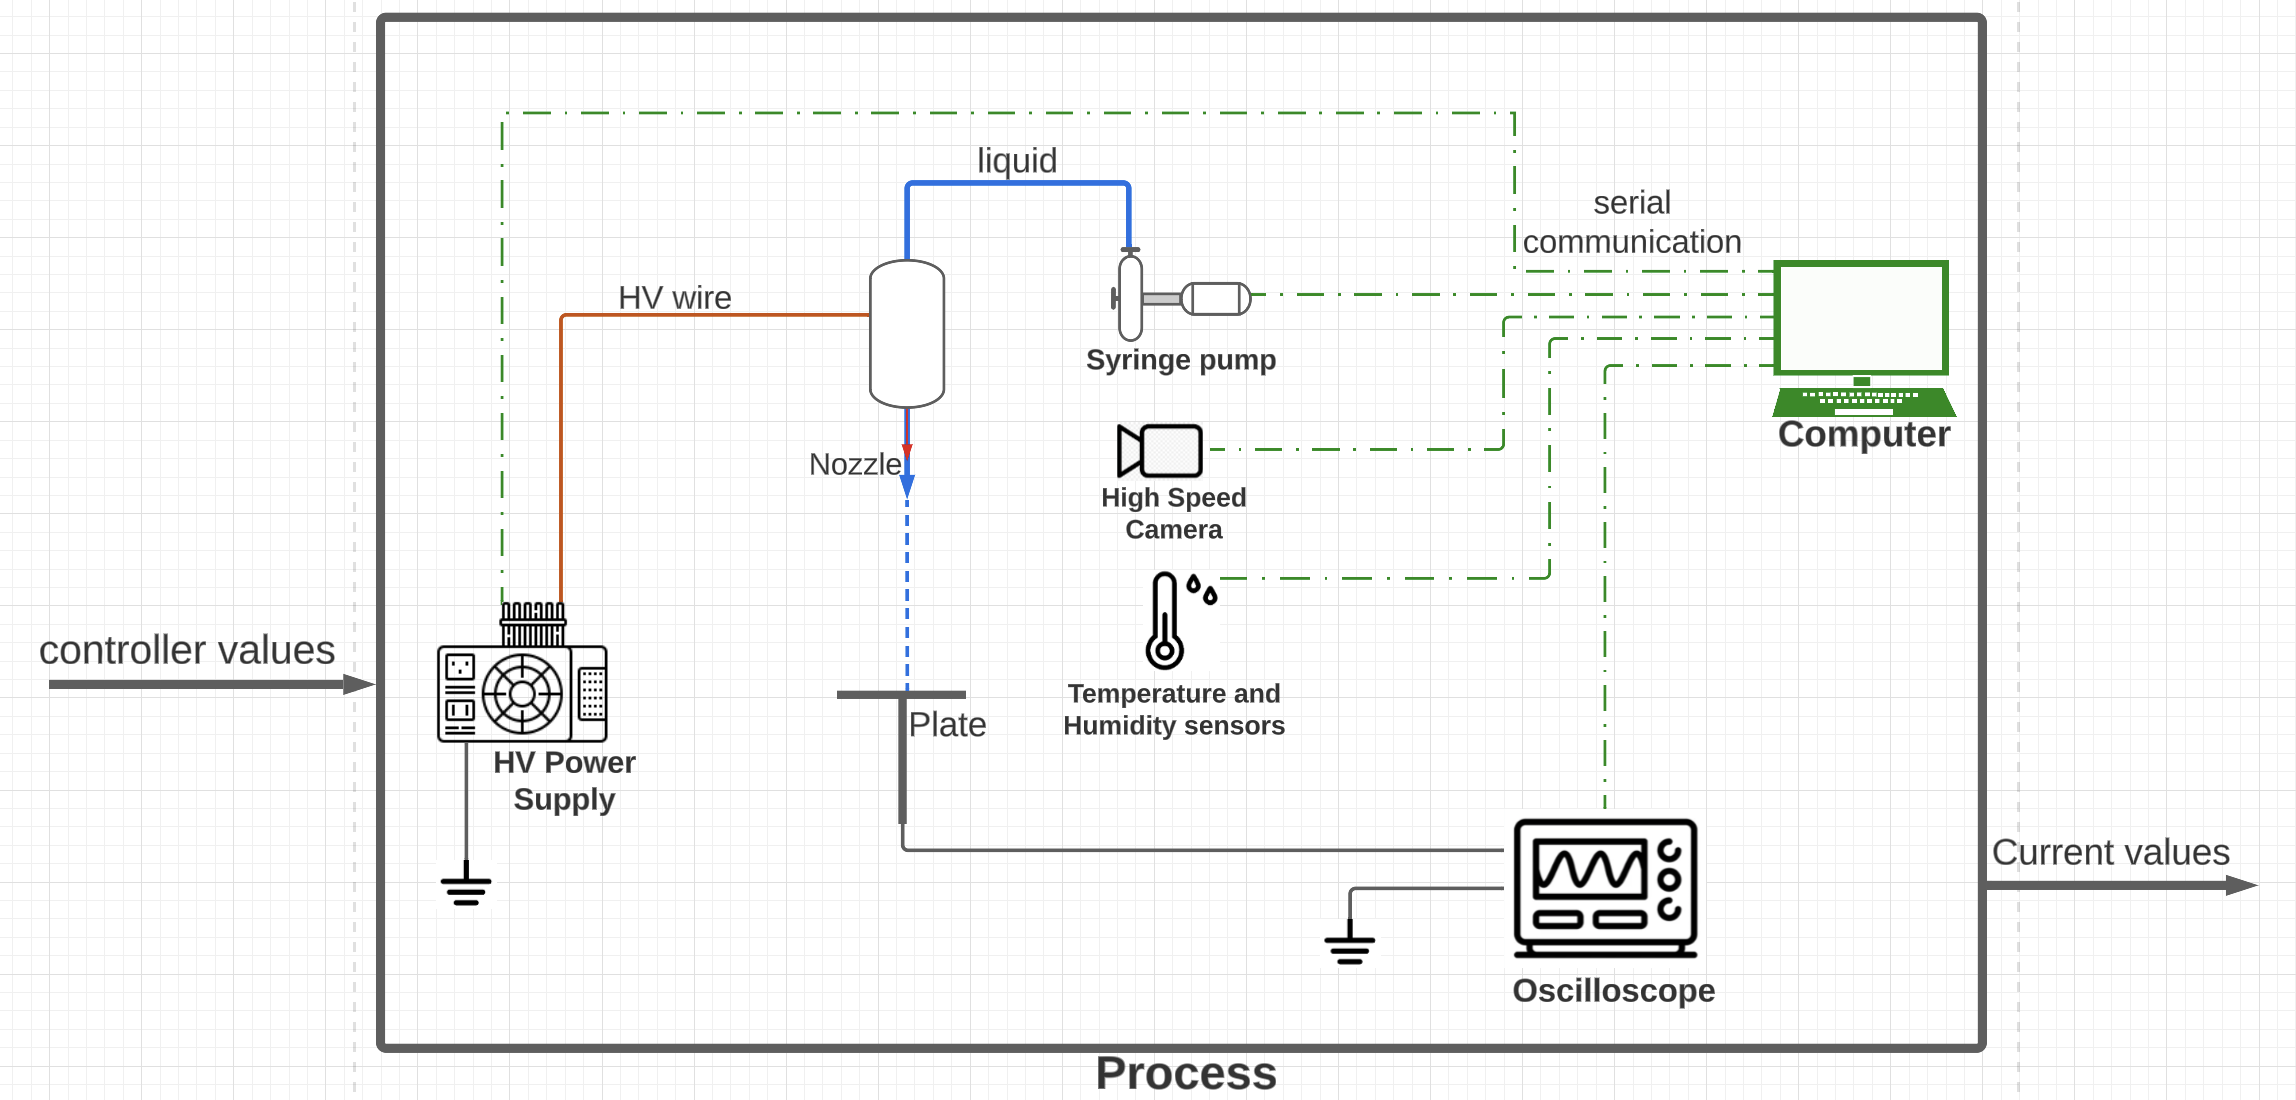
\includegraphics{systemDescription/Figuras/new_system_setup.png}}
  \caption{EHDA automation system setup}
  \label{fig:setup}
\end{figure}


\section{section title}
\label{sec:revisão}


\clearpage
